\chapter{Outlining Story centric Brainstorming and Collaboration }
\label{chap_anatomy}

This thesis proposes a system for story-centric distributed brainstorming and collaboration. Story-centric collaborations between makers and nonprofits are collaborations that are a result of the stories told by nonprofits. These stories represent the goals, processes and constraints of the nonprofits. While these nonprofits will not always have the expertise to define a challenge a specification of a solution, they are well versed in their story.

Before designing a distributed system it is crucial to understand how these type of collaborations work in small scale. To that purpose I present three case studies of story centric brainstorming and collaboration. These case studies are based on testimonials from relevant organizations and participants through unstructured interviews. At the end of the Chapter I present my impressions and a common process extracted from these cases. 

\section{Milky}
This case study represents my own experience in working with the Mothers' Milk Bank Northeast \cite{mmne}. This collaboration started in the summer of 2015, before my thesis research started, and served as motivation for the research direction I chose.

The Mothers' Milk Bank Northeast is a non profit community organization that receives donations of human milk, processes them and provides them to babies in fragile health throughout the Northeastern United States. Breast milk is considered to be the healthiest source of nutrients for babies and especially important in cases of preterm birth, infectious disease and various other medical conditions.\cite{} However, for various reasons, sometimes the birth mother can not lactate. The milk bank collects donated milk and makes it available through hospitals. 

I learned about the milk bank completely by chance. My peer, Tal Achituv, had co-organized a hackathon which was dedicated to the improvement of breast milk pumps \cite{d2016feminist}. One of the attendees, Yavni Bar-Yam, was the son of Naomi Bar-Yam, who runs the milk bank. Yavni told Tal about the organization, who in turn convinced me to come for a visit. I had just finished my first year as a grad student at the media lab and had an itch for industrial design and hardware fabrication.

In the visit, we learned about the process breast milk donations go through from collection until being received in hospitals. This included processing of the milk: mixing it, pasteurizing and bottling. One of the things we noticed was that the tools used by the lab workers were very basic. The milk was hand poured through a series of vessels and finally into the bottles, where the main measurement tool was eyeballing the volume markings. 

   \begin{figure}[thpb]
      \centering
      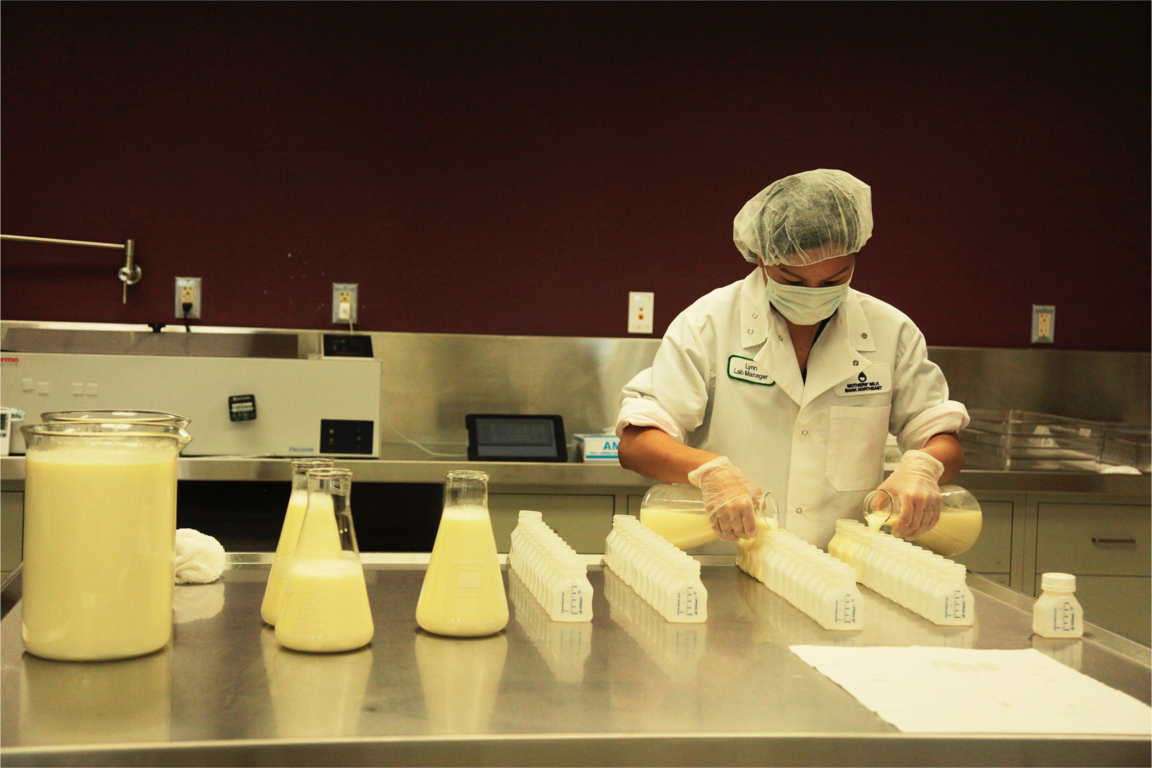
\includegraphics[width=4in]{figures/mmne-manual.png}
      \caption{Manual pouring of milk in Mothers' Milk Bank Northeast}
      \label{mmne-manual}
   \end{figure}

This manual process became the focal point of our discussion. While it was cumbersome it also presented issues of accuracy and being prone to infections. The milk bank had tried to address these issues before using an off the shelf peristaltic pump instead of manually pouring. However, it slowed down the pace of work and did not allow for parallelization between lab workers. 

We suggested a simple solution for the problem, building a carousel bottle feeder in conjunction with a peristaltic pump. The carousel will allow continuous feeding of empty bottles on one side and capping and removing the bottles on the other side. We called this device Milky. 

   \begin{figure}[thpb]
      \centering
      \includegraphics[width=4in]{figures/milky.png}
      \caption{Milky - Early Prototype}
      \label{milky}
   \end{figure}

We built several iterations of Milky during a period of several months while being in constant dialog with Milk Bank. We did so in collaboration with the organization's employees. The lab workers, who will eventually use the machine, gave us feedback early along the process to make sure the device fits in the lab and is suitable for their work flow. David, consulted us regarding materials, sanity and made sure that the process does not prove to be harmful for the milk. 

Milky itself hasn't been deployed due to the delicate nature of the operation and a necessity for continuous on site support requirements. However, the continued process of brainstorming and collaboration has led the milk bank to commission an industrial quality version of it from a local engineering firm. The specification for this machine were outlined in collaboration with us, based on the insights from our continuous brainstorming and experimentation process. This machine is scheduled for deployment on September 2016.

For me, this was an invaluable experience. I got a chance to utilize my newly acquired skills and have a real world impact.  In developing Milky, I became convinced that there is an unrealized opportunity for makers and nonprofits to collaborate in a way that could be beneficial for both parties.

\section{Laser Painting}

Deborah Dawson, an artist from New York, helps kids with cerebral palsy to create art. She does so by attaching a small laser pointer to their heads and have them point at a painting canvas. In turn, she traces their pointer to create an abstract painting. This allows kids with very little ability to express themselves, to create art they can call their own.

   \begin{figure}[thpb]
      \centering
      \includegraphics[width=4in]{figures/laser-session.png}
      \caption{Deb Dawson in a Laser Painting session}
      \label{laser-session}
   \end{figure}

However, Deb had a challenge with mounting these devices. Laser pointers are not designed to be worn on the head. This proves to be very difficult, especially by kids that suffer from cerebral palsy and have limited motor skills. Her quest to find a more suitable alternative led her to companies that manufacture lasers sights built for guns. Naturally, these companies could not help. Eventually, on a long shot, she sent an email describing her issues to an MIT Media Lab Prof., Ros Picard, who in turn sent it to all Media Lab students (see Appendix). 

Tal Achituv, spotted that email and invited Deb to MIT. Deb, Tal and several other students, including myself, met with her. We learned about her work and suggested a headband design with an integrated low power laser pointer for the kids. Moreover, through our conversation we learned about her entire operation which led to a discussion over some other challenges she faces. For example, the fact the she worked in different schools and in different spaces meant that all the equipment needed to be carried around. Not to mention, locating spaces that had the accessibility requirements for these kids was also challenging. One of the ideas we discussed was repurposing an old school bus with wheelchair accessibility and the painting infrastructure. That way the equipment only needs to be setup once and the bus could travel around New York and cater to various schools in different locations. 

   \begin{figure}[thpb]
      \centering
      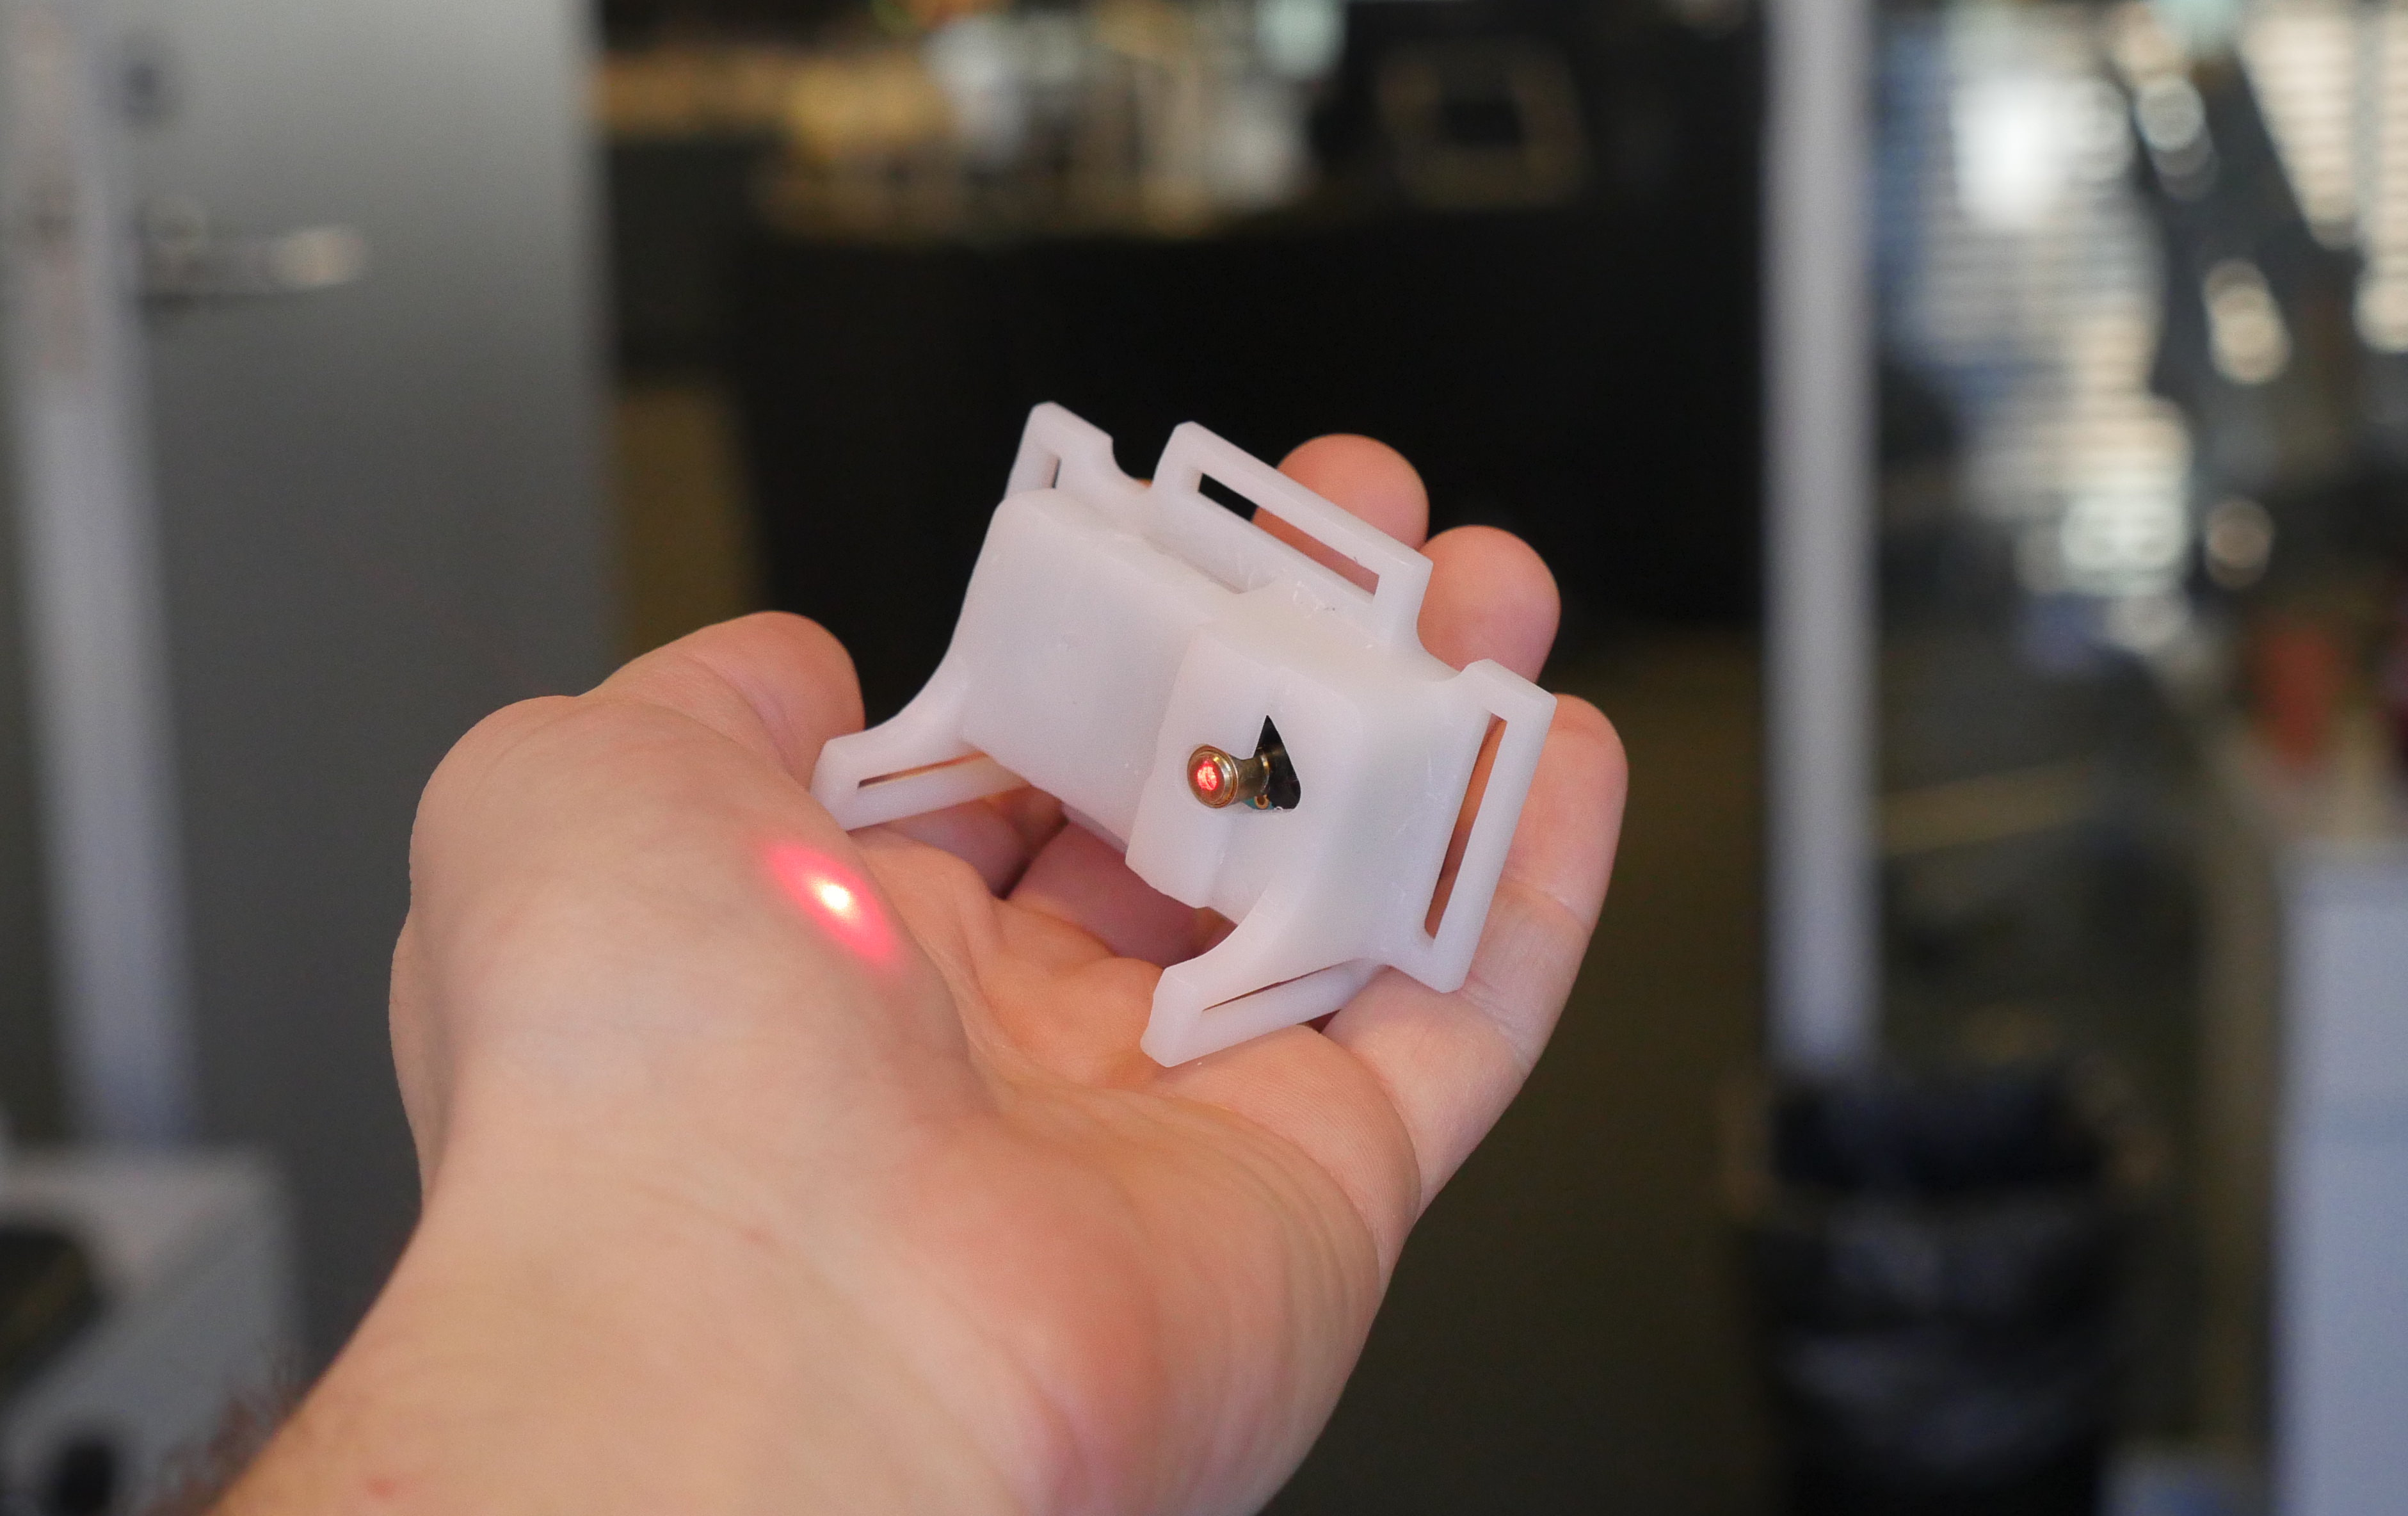
\includegraphics[width=4in]{figures/new-laser.jpg}
      \caption{Improved Laser apparatus for Laser Painting. Includes a safe low power laser and a various mounting options.}
      \label{new-laser}
   \end{figure}


The alternative headband laser pointer was delivered to Deb in the Spring of 2016 and has been in use since then. Moreover, Deb is currently looking to expand her operations and is in touch with maker spaces in New York to fabricate more of them. Also, Deb is actively seeking funding for the re-purposing of a bus as a portable studio for her work. 

This collaboration has also inspired Tal to further explore the world of assisted self expression.  For his thesis project he built a painting machine that assists people with various disabilities to express themselves by drawing, with minimal assistance from other people\cite{projexpress}. 

   \begin{figure}[thpb]
      \centering
      \includegraphics[width=4in]{figures/express.png}
      \caption{Project \textit{Express} - Self assisted painting machine}
      \label{express}
   \end{figure}

From this collaboration I learned that while nonprofits will often seek help with a small, narrow challenge, there is an opportunity for both parties in discussing the bigger picture: the story. 

\section{Cradles to Crayons}

Following the previous two study cases, I set out to initiate a more structured exploration into the space. In contrast to our previous experiences, which happened completely by chance, this time I actively sought out a potential collaboration. 

The initial challenge was to find a suitable organization. Given that nonprofit organizations matched the profile, I approached the Massachusetts Nonprofit Network (MNN). The MNN agreed to publish a call for collaboration in their weekly newsletter which yielded some 50 requests from various nonprofits (see Appendix). In the requests, one stood out as having a complex ground operation that might be of interest to makers, Cradles to Crayons.   

Cradles to Crayons (C2C) provides children from birth to age 12, living in low-income and homeless situations, with the essential items they need to thrive – at home, at school and at play. They supply these items free of charge by engaging and connecting communities that have with communities that need.

The C2C operation is a complex logistic one. It starts with donation bins distributed in local communities and goes through sorting and filtering in their main facility, and ends in creating custom packs for children in need, which are distributed through local social workers. 

I arranged for a party of 15 makers to visit the C2C facility in Brighton, MA. These were reached through my personal network at the Media Lab and maker-spaces in Boston, they expressed interest in learning about nonprofits and their skills varied from Software Engineering to Mechanical Engineering and Art. The tour was led by Julia Boyaval, director of community engagement for C2C, who received no instructions apart from showing around the facility the same way she would in any other circumstance. During the tour the participants learned about the different challenges the organization faces: from the security of their donations bins to difficulties of managing stock. This learning process was backed by a continuous discussion between the participants, Julia and other employees of the organization. 

   \begin{figure}[thpb]
      \centering
      \includegraphics[width=4in]{figures/c2c-tour.jpg}
      \caption{A Maker tour of Cradles to Crayons}
      \label{fig_setc_class}
   \end{figure}

At the end of the tour the participants gathered in an office to discuss. Given that C2C have a complex operation, the first thing they did is formalize the entire operation as a block diagram on a whiteboard, utilizing one of the participants as a moderator. Next, each participant was given a sticky note to write one idea on, and stick it on the whiteboard around the most relevant block. This quickly formed clusters of sticky notes around identified blocks and triggered a discussion about the different problems and the various proposed solution. 

   \begin{figure}[thpb]
      \centering
      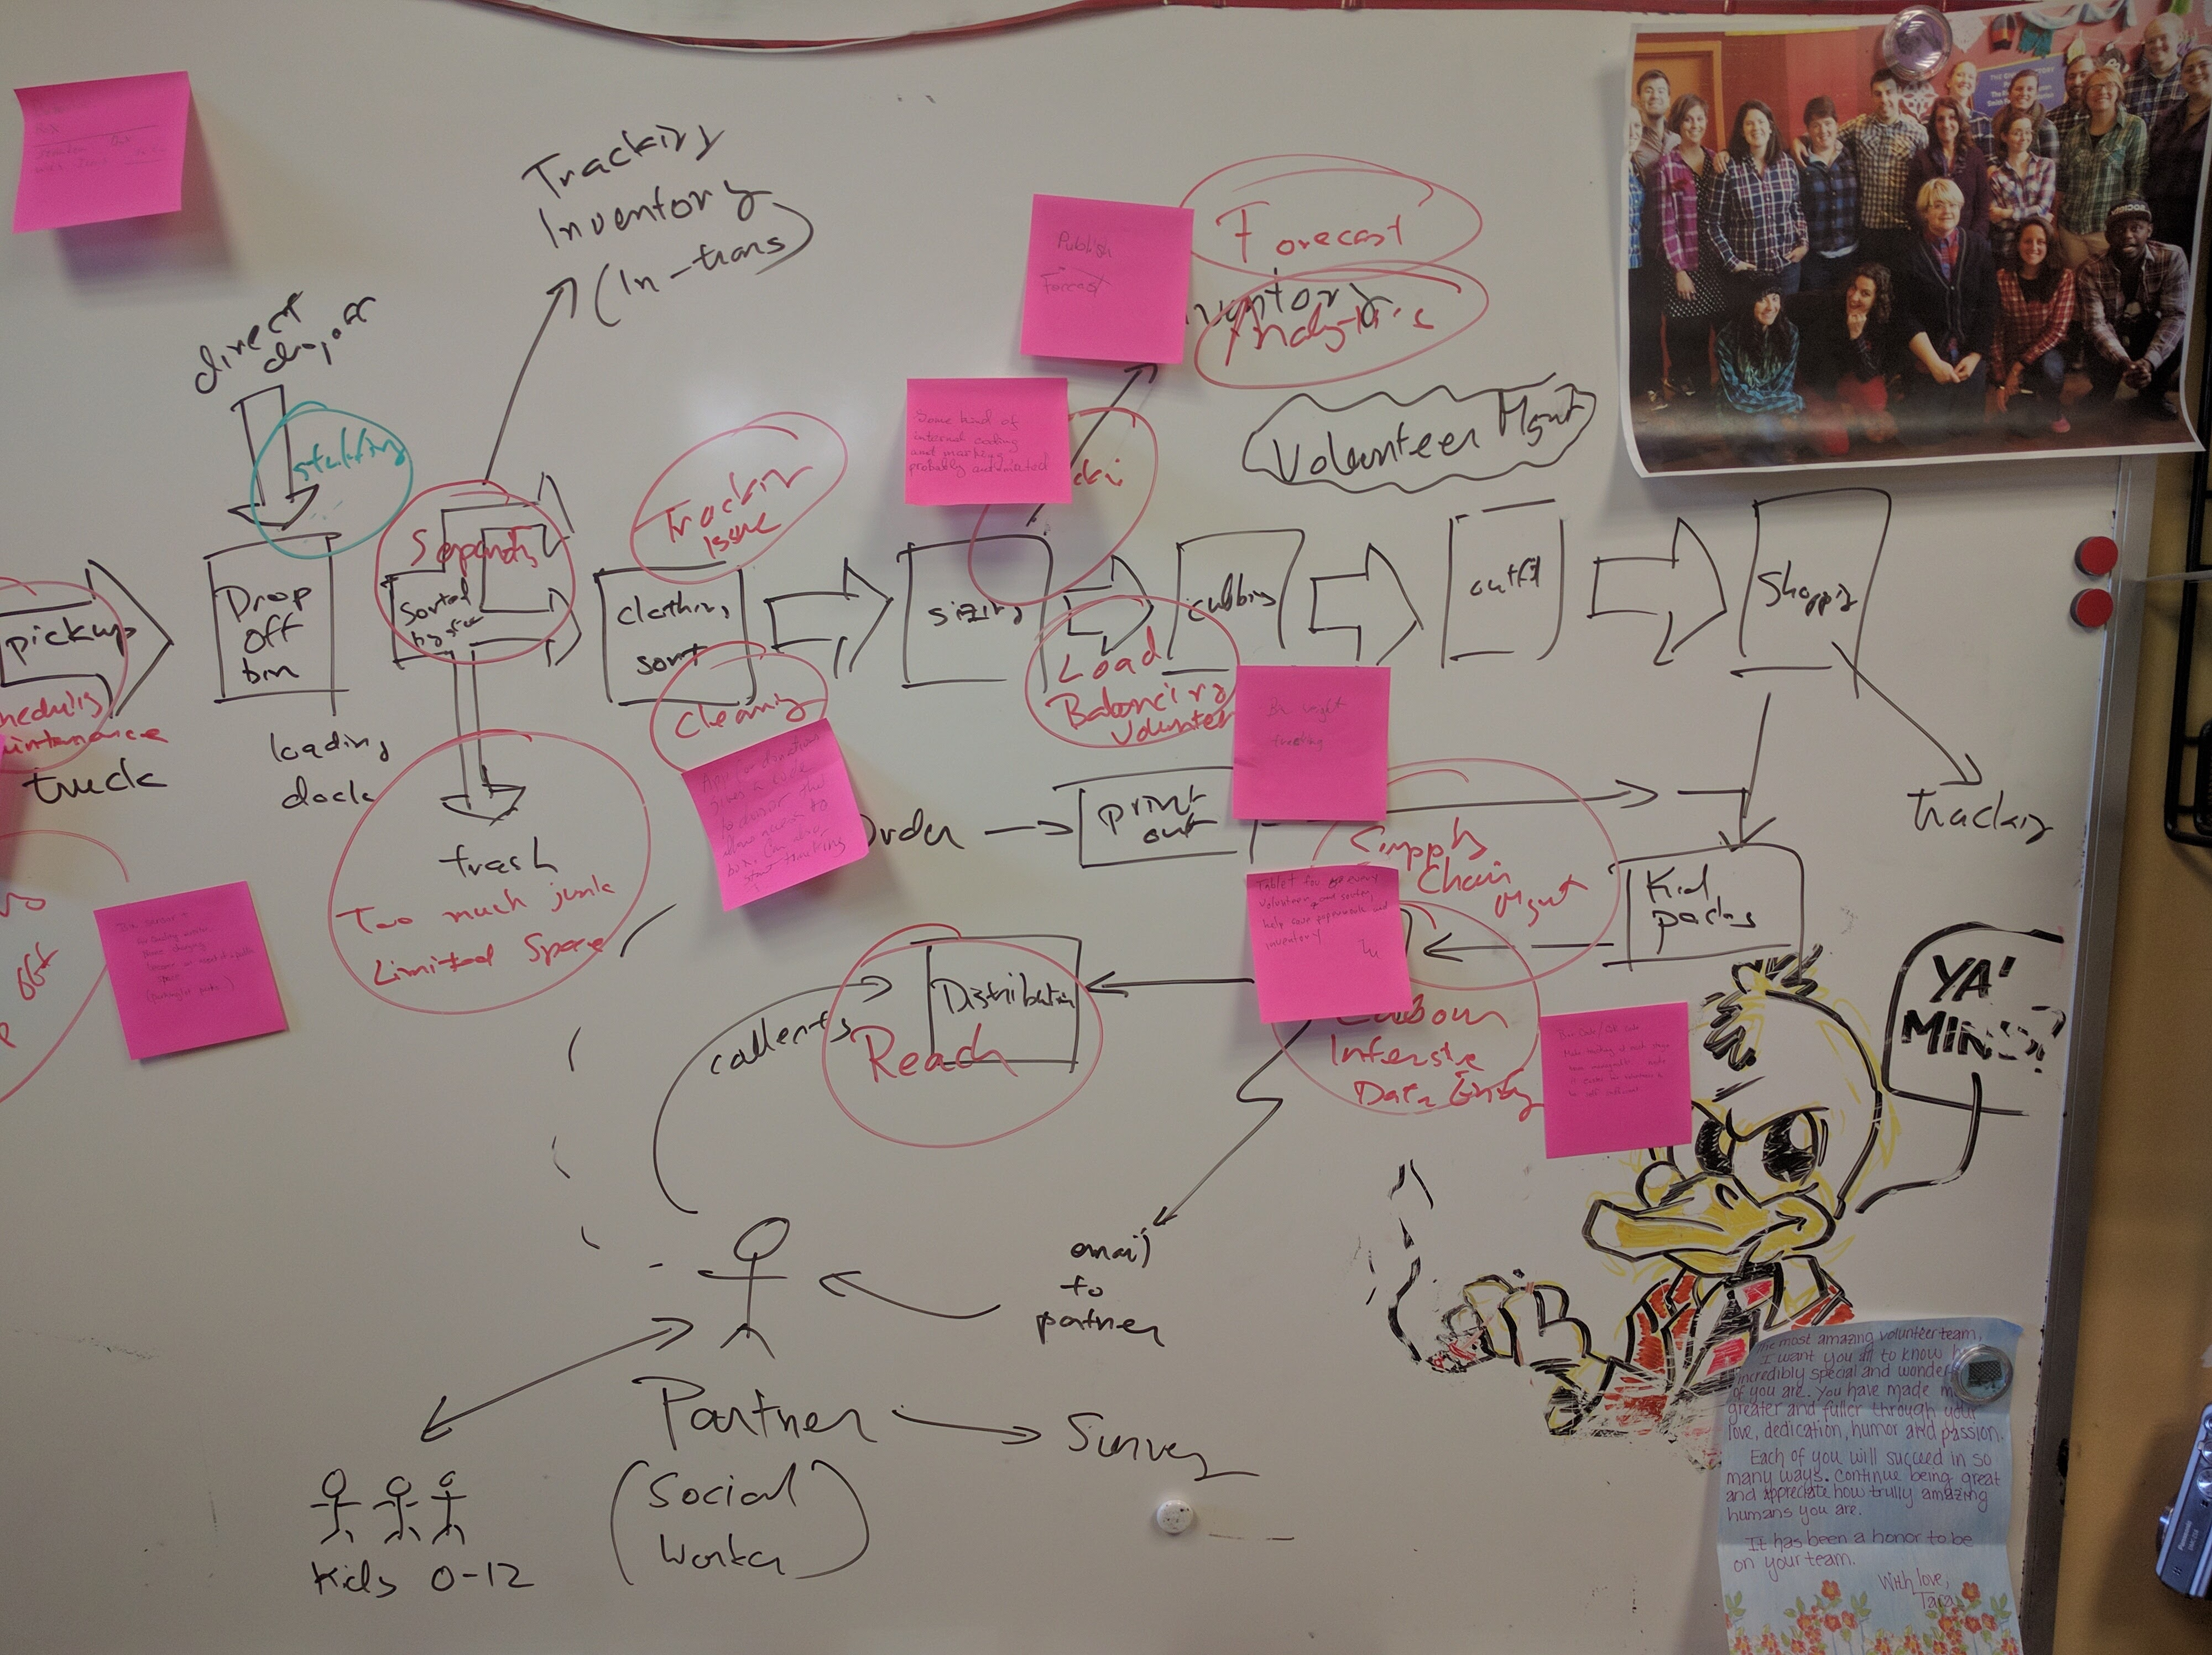
\includegraphics[width=4in]{figures/c2c-brainstorming.jpg}
      \caption{Whiteboard post Cradles to Crayons brainstorming session}
      \label{fig_setc_class}
   \end{figure}


The proposed ideas varied in nature. One of them, a mobile application, tackled the inventory issues by allowing donors to create a manifest of their donations in advance. Another, suggested creating a direct link, using a mobile app, between the donors and the social workers, thus reducing congestion in the facility. Others were as simple as modifying the graphics on the bins to better instruct the donors what belongs in them and what doesn't. 

At the end of the tour several of the participants expressed interest in working with C2C although none of them is currently engaged in such collaboration, citing time constraints as the main barrier. With that said, the event was still successful as the idea of creating a direct link between donors and social workers through a mobile app has been approved by management and is in an initial phase of implementation by the organization. The congestion challenge this app addresses was not part of the challenges originally laid out by Julia but rather surfaced from the broad story of the organization, showing the power of these stories.  

This exploratory collaboration has taught me about the different nature of nonprofits. While the previous two case studies addressed small nonprofits, C2C is a different story. They are a national nonprofit with close to hundred employees, three large scale distribution centers and tens of thousands of donation packages processed per week. At such a scale, experimenting is non-trivial and failed experiments might lead to public relation issues. 

\section{Impressions}

Examining the above cases demonstrate that the concept of story-centric brainstorming and collaboration works towards the goals I stated in the introduction chapter. All the nonprofits mentioned have stated that they have gained a valuable different perspective on the challenges they're facing while learning about the abilities and skill sets of the makers they've worked with. In turn, the makers learned about the different operations of these nonprofits and how their skill sets can help improve them. Even in cases where the collaboration itself has not produced a successful artifact, they still had an significant impact on all parties involved. 

\section{Formalizing the process}

Based on these three case studies I present a common process that has three phases. While these cases focus on nonprofit organizations and participants with background in engineering, there is still some variance in the different challenges and nature of collaboration. I believe this process is generalized enough to be used to tackle various challenges with different organizations and participants. 

\begin{enumerate}

\item \textit{Discovery} - Discovery is perhaps the most elusive step of this process but is a basic requirement for it's existence. In the two first cases discovery happened completely by chance while the third one was the result of an intended search. How do organizations learn about the existence of these type of participants and vice versa? Moreover, how do you encourage them to engage with one another? 

\item \textit{Exploration} - In all of the above cases, participants had at least one on-site visit with the respective organizations. These explorations started from a general overview and ended in a detailed drill down into the processes employed by the organization. Open discussion during this exploration proves to be a major role in understanding the organization: motivation, processes and constraints. 

\item \textit{Collaborative Brainstorming} - The next step in all of these examples is a process of collaborative brainstorming. This included tossing around many ideas and, filtering and refining them according to the given constraints. These sometimes began in a spontaneous meeting right after the exploration phase but also went on to remote forms of communications be it phone, email etc.

\item \textit{Co-design} - This final step represents an ongoing relationship of design and refinement in which a prototype is built by makers, evaluated with the nonprofit and so forth. This process is present in the first two case studies examined yet is absent from the third. While initially it may seem like the most important step, the case studies show that that there is still significant value in the process without it. 

\end{enumerate}
 
Having established that these type of collaborations work towards the goals I stated, the next challenge is to translate the outlined process into an online experience that can be scaled while preserving the unique properties of the real life experience. From here on, I will focus on the first three steps of the outlines process given that they provide a basis for collaboration and have shown to provide value on their own.